% --------------------------------------------------------------------------- %
% Poster for the ECCS 2011 Conference about Elementary Dynamic Networks.      %
% --------------------------------------------------------------------------- %
% Created with Brian Amberg's LaTeX Poster Template. Please refer for the     %
% attached README.md file for the details how to compile with `pdflatex`.     %
% --------------------------------------------------------------------------- %
% $LastChangedDate:: 2011-09-11 10:57:12 +0200 (V, 11 szept. 2011)          $ %
% $LastChangedRevision:: 128                                                $ %
% $LastChangedBy:: rlegendi                                                 $ %
% $Id:: poster.tex 128 2011-09-11 08:57:12Z rlegendi                        $ %
% --------------------------------------------------------------------------- %
\documentclass[a0paper,landscape]{baposter}

\usepackage{relsize}		% For \smaller
\usepackage{url}			% For \url
\usepackage{epstopdf}	% Included EPS files automatically converted to PDF to include with pdflatex
\usepackage{natbib}
\usepackage{paralist}
\usepackage{wrapfig}
\usepackage[font=small,labelfont=bf]{caption}
%%% Global Settings %%%%%%%%%%%%%%%%%%%%%%%%%%%%%%%%%%%%%%%%%%%%%%%%%%%%%%%%%%%

\graphicspath{{./}}	% Root directory of the pictures 
\tracingstats=2			% Enabled LaTeX logging with conditionals

%%% Color Definitions %%%%%%%%%%%%%%%%%%%%%%%%%%%%%%%%%%%%%%%%%%%%%%%%%%%%%%%%%

\definecolor{bordercol}{RGB}{0,0,0}
\definecolor{headercol1}{RGB}{186,186,186}
\definecolor{headercol2}{RGB}{90,110,200}
\definecolor{headerfontcol}{RGB}{0,0,0}
\definecolor{boxcolor}{RGB}{225,225,225}

%%%%%%%%%%%%%%%%%%%%%%%%%%%%%%%%%%%%%%%%%%%%%%%%%%%%%%%%%%%%%%%%%%%%%%%%%%%%%%%%
%%% Utility functions %%%%%%%%%%%%%%%%%%%%%%%%%%%%%%%%%%%%%%%%%%%%%%%%%%%%%%%%%%

%%% Save space in lists. Use this after the opening of the list %%%%%%%%%%%%%%%%
\newcommand{\compresslist}{
	\setlength{\itemsep}{1pt}
	\setlength{\parskip}{0pt}
	\setlength{\parsep}{0pt}
}

%%%%%%%%%%%%%%%%%%%%%%%%%%%%%%%%%%%%%%%%%%%%%%%%%%%%%%%%%%%%%%%%%%%%%%%%%%%%%%%
%%% Document Start %%%%%%%%%%%%%%%%%%%%%%%%%%%%%%%%%%%%%%%%%%%%%%%%%%%%%%%%%%%%
%%%%%%%%%%%%%%%%%%%%%%%%%%%%%%%%%%%%%%%%%%%%%%%%%%%%%%%%%%%%%%%%%%%%%%%%%%%%%%%

\begin{document}
\typeout{Poster rendering started}

%%% Setting Background Image %%%%%%%%%%%%%%%%%%%%%%%%%%%%%%%%%%%%%%%%%%%%%%%%%%
\background{
%	\begin{tikzpicture}[remember picture,overlay]%
%	\draw (current page.north west)+(-2em,2em) node[anchor=north west]
%	{\includegraphics[height=1.1\textheight]{background}};
%	\end{tikzpicture}
}

%%% General Poster Settings %%%%%%%%%%%%%%%%%%%%%%%%%%%%%%%%%%%%%%%%%%%%%%%%%%%
%%%%%% Eye Catcher, Title, Authors and University Images %%%%%%%%%%%%%%%%%%%%%%
\begin{poster}{
	grid=false,
	% Option is left on true though the eyecatcher is not used. The reason is
	% that we have a bit nicer looking title and author formatting in the headercol
	% this way
	eyecatcher=true, 
	borderColor=bordercol,
	headerColorOne=headercol1,
	headerColorTwo=headercol2,
	headerFontColor=headerfontcol,
	% Only simple background color used, no shading, so boxColorTwo isn't necessary
	boxColorOne=boxcolor,
	headershape=roundedright,
	headerfont=\Large\sf\bf,
	textborder=rectangle,
	background=user,
	headerborder=open,
  boxshade=plain
}
%%% Eye Cacther %%%%%%%%%%%%%%%%%%%%%%%%%%%%%%%%%%%%%%%%%%%%%%%%%%%%%%%%%%%%%%%
{
\includegraphics[width=6em,height=6em]{jayhawk}
}
%%% Title %%%%%%%%%%%%%%%%%%%%%%%%%%%%%%%%%%%%%%%%%%%%%%%%%%%%%%%%%%%%%%%%%%%%%
{\bf
	Algorithms for Calculating Parsimony-Uninformative Pattern Class Probabilities on Trees
}
%%% Authors %%%%%%%%%%%%%%%%%%%%%%%%%%%%%%%%%%%%%%%%%%%%%%%%%%%%%%%%%%%%%%%%%%%
{
	\vspace{0em} Jordan M. Koch and Mark T. Holder\\
}
%%% Logo %%%%%%%%%%%%%%%%%%%%%%%%%%%%%%%%%%%%%%%%%%%%%%%%%%%%%%%%%%%%%%%%%%%%%%
{
% The logos are compressed a bit into a simple box to make them smaller on the result
% (Wasn't able to find any bigger of them.)

\setlength\fboxsep{0pt}
\setlength\fboxrule{0.5pt}
%	\fbox{
%		\begin{minipage}{6em}
			%\includegraphics[width=10em,height=4em]{colbud_logo}
			%\includegraphics[width=4em,height=4em]{elte_logo} \\
			%\includegraphics[width=10em,height=4em]{dynanets_logo}
			\includegraphics[width=6em,height=6em]{imsdlogo}
%		\end{minipage}
%	}
}

\headerbox{Abstract}{name=intro,column=0,row=0}{
A wide variety of evolutionary analyses are based upon the pairing of phylogenetic trees
with models of how biological traits change during evolution.
In some contexts, one needs to calculate the probability that any member of a class of
 patterns will arise on the tree.
 For example, the model adequacy approach of Waddell et al. (2009) requires calculating 
 the probability of several classes of patterns. 
 In order to extend Lewis's (2001) morphological models to deal with many data sets, 
 calculating the probability of any parsimony-informative pattern arising is required
 (`parsimony' referring to the simplest explanation of the data, and 
 `parsimony-informative' referring to those patterns which affect phylogenetic estimation). 
 \vskip 1em
We recently published an algorithm that includes a general approach applicable to any 
standard model of character evolution \cite{KochH2012}.  
We validated our data against Waddell's simulations, and performed run-time performance tests.
Now, we are working to develop efficient, dynamic programming algorithms, which calculate the 
probabilities of a parsimony-uninformative pattern in one pass down a phylogenetic tree.
Allman {\em et al.~}\cite{AllmanHR2010} showed that trees could be estimated from datasets that filtered to 
contain only parsimony sites, if one can correct for the data filtering.
This requires the calculation of the probability of generating a parsimony-uninformative
pattern.
We are now implementing these algorithms in open-source software written in C++.
We plan to include the approaches in the GARLI software package for use in inferring evolutionary trees.
 \vskip 0.5em
%
}

\headerbox{Research Goals}{name=research goals,column=0,below=intro}{
\begin{compactenum}
\item Develop specialized algorithms for calculating the probability of a parsimony-uninformative character.
 \vskip .67em
\item Implement the algorithms into testing software in C++
 \vskip .67em
\item Add the algorithms to GARLI for use in phylogenetic inference
(Recognizing these symmetric cases will make the code run more efficiently and accurately in C++).
 \vskip 0.5em
\end{compactenum}
}i

\headerbox{A General Algorithm for Classes Based on Parsimony Length}{name=results,span=2,column=1,row=0}{
%\begin{wrapfigure}{r}{25em}
%	\vskip -1.5em
%		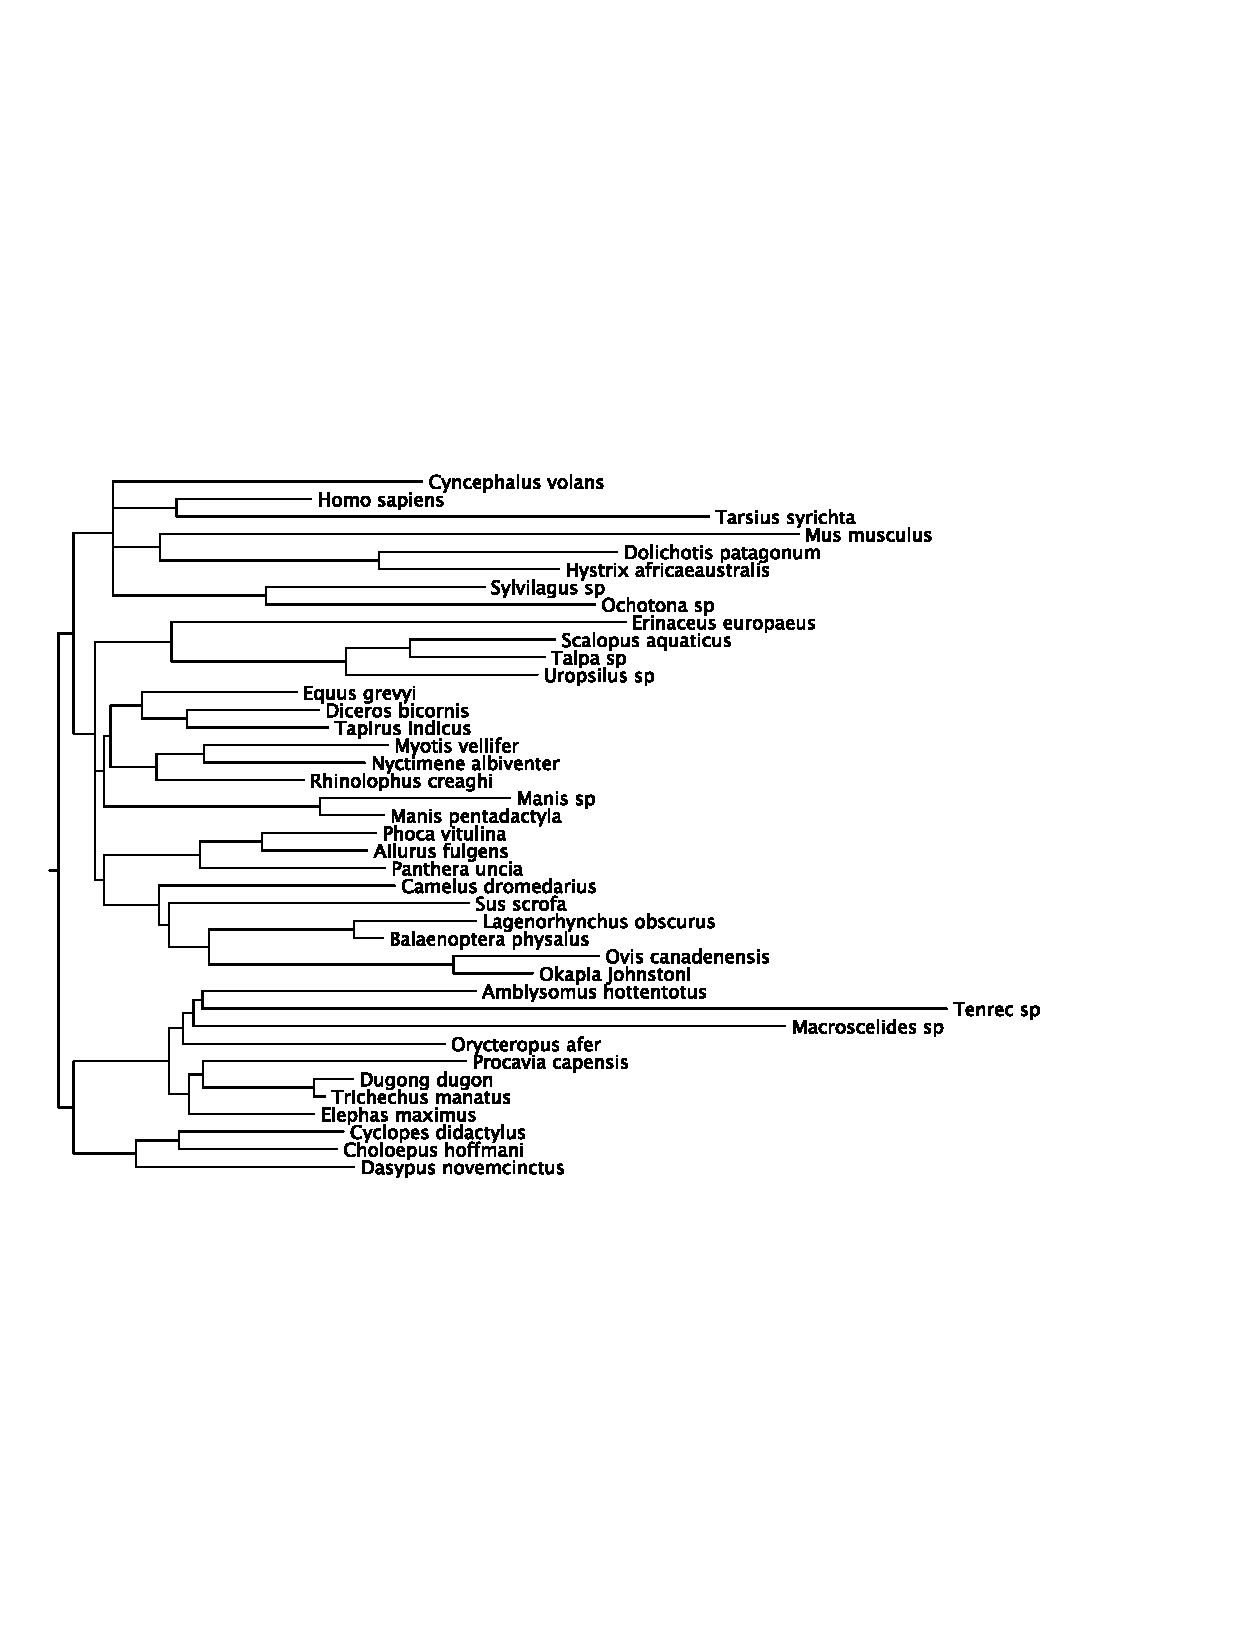
\includegraphics[width=25em]{waddellTree}
%	\vskip -.5em
%		\caption{Gene tree for RAG-1 sequences used by Waddell {\em et al.~}\citep{WaddellOP2009}. Branch lengths are shown in proportion to the expected number of changes per site. Our algorithm can calculate quantities such as ``the probability of a character evolving on this tree and showing states A and C and a parsimony length of 5''}\label{waddellTreeFig}
%	\vskip -1.0em
%\end{wrapfigure}
\begin{wrapfigure}{r}{15em}
	\vskip -1.5em
		\includegraphics[width=15em]{Log2RunTimeGraph}
	\vskip -.5em
	\caption{Computational time as a function of number of tips in a tree.  Given a fixed tree with branch lengths and values for the parameters of the GTR (general time reversible) model, we can report the probabilities of pattern classes for nucleotide data.
	%Combinations of state-sets for left and right child which lead to downpass state set of $\{0\}$ when $k=3$. In the fully symmetric case, edges shown with the same color are guaranteed to have the same probability. There are 9 edges, but only 6 colors.
	}\label{Log2RunTimeGraph}
\end{wrapfigure}
The model adequacy assessment \citep{WaddellOP2009} and the extension of Lewis's \citep{Lewis2001} model both entail calculations based on classes of patterns that share the same parsimony length on a tree.
The model adequacy test also requires partitioning patterns based on the set of states observed at the leaves of the tree.
%Fitch \citep{Fitch1971} provided an efficient algorithm for calculating the parsimony score.
\begin{wrapfigure}{l}{20em}
\begin{tabular}{|cc|c|c|}
\hline
\# & \#  & Waddell's  & Our \\
 steps & states & simulation &  algorithm\\
\hline
0 & 1 & 282 & 283.21\\
1 & 2 & 110.1 & 109.00\\
2 & 2 & 48.0 & 48.60\\
3 & 2 & 25.5 & 24.67\\
4 & 2 & 12.9 & 12.59\\
5 & 2 & 6.6 & 6.30\\
6 & 2 & 3.1 & 3.09\\
%7-20 & 2 & 2.5 & 2.59\\
%2 & 3 & 40.3 & 40.26\\
%3 & 3 & 38.2 & 38.43\\
%4 & 3 & 29.7 & 29.98\\
%5 & 3 & 21.8 & 21.51\\
%6 & 3 & 14.4 & 14.70\\
%7 & 3 & 9.7 & 9.63\\
%8 & 3 & 5.7 & 5.94\\
%9 & 3 & 3.2 & 3.35\\
%10-26 & 3 & 2.8 & 2.80\\
%3-4 & 4 & 16.8 & 16.43\\
%5 & 4 & 11.4 & 11.39\\
%6 & 4 & 11 & 11.32\\
%7 & 4 & 10.3 & 10.29\\
%8 & 4 & 8.2 & 8.61\\
%9 & 4 & 6.5 & 6.50\\
%10 & 4 & 4.3 & 4.31\\
%11-30 & 4 & 4.7 & 4.51\\
\hline
\end{tabular}
\caption{Comparison of the expected number of sites simulated by Waddell et al. to the expected number of sites calculated by our algorithm.  The closeness between the respective values shows our algorithm to be valid.}\label{ComparisonToWaddell}
\vskip 1.5em
\end{wrapfigure}
%The Fitch algorithm can calculate the parsimony length for a tree rooted at an internal node from a ``downpass state set'' for the children of the node.
We have developed a dynamic programming algorithm that can calculate the probability of classes of patterns that share the same set of observed states and parsimony length on a tree. For a tree of $N$ leaves, the algorithm requires storing bins of probability for:
\begin{compactitem}
	\item each of the $N-1$ internal nodes,
	\item each of the $\approx N - 1$ parsimony lengths,
	\item each of the $k$ ancestral states,
	\item  each of the $2^{k}-1$ observed state sets, and
	\item each of the $2^{k}-1$ downpass state sets in Fitch's \cite{Fitch1971} algorithm.
\end{compactitem}
yielding an approximate memory requirement of $\mathcal{O}(N^2 k 2^{2k}$).
$k$ is bounded and often small ($k=4$ for DNA data).
With respect to tree size, calculations scale $\mathcal{O}(N^3)$ (see Figure \ref{Log2RunTimeGraph})
Waddell {\em et al.~}\citep{WaddellOP2009} used simulation on a tree of mammals to obtain probabilities for classes of patterns.
We validated our algorithm with the same data and confirmed very similar probability calculations (Figure \ref{ComparisonToWaddell}).  
These results were presented in our recently published article in the PloS Currents Tree of Life online journal\cite{KochH2012}.


%}
%\headerbox{Specializing for the Symmetric Models}{name=results2,span=2,column=1,below=results}{
%\begin{wrapfigure}{r}{15em}
%	\vskip -1.5em
%		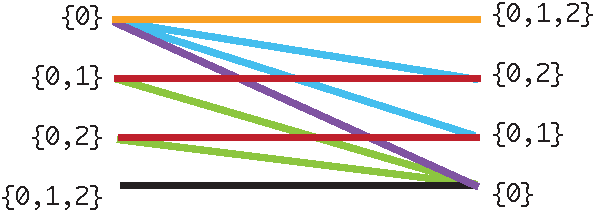
\includegraphics[width=15em]{downpass-symmetry-small}
%	\vskip -.5em
%	\caption{Combinations of state-sets for left and right child which lead to downpass state set of $\{0\}$ when $k=3$. In the fully symmetric case, edges shown with the same color are guaranteed to have the same probability. There are 9 edges, but only 6 colors.}\label{symmetryFig}
%\end{wrapfigure}
\vskip 1em \large \textbf{Specialization for parsimony-uninformative patterns}\normalsize\\
\vskip .5em
For decades, the parsimony method was the dominant means of inferring phylogenies from
morphological data. 
Thus many datasets describing morphological traits of organisms will contain only patterns 
which are parsimony-informative.
Correcting for this filtering of data to only include parsimony informative patterns
is crucial to reliable tree inference \cite{NylanderRHN2004,AllmanHR2010}.
To correct the calculations, one must be able to calculate the probability of 
generating a parsimony uninformative pattern.

We are in the last stages of developing a specialization of the algorithm for calculating the class of parsimony uninformative patterns.
By definition, a parsimony informative pattern will a length of $k-1$, thus we do not need to keep probabilities
for an array of tree lengths.
We can also ignore the $\mathcal{O}(2^{k}$) downpass states, in lieu of recording which of the $k$ states is repeated in the tree (there can only be one repeated state in a parsimony-uninformative site). 
Thus the specialization should have memory requirements that scale as $\mathcal{O}(N k^2 2^{k}$).

The need to consider multiple parsimony lengths as well as consider all possible ways of partitioning this length between the left and right subtrees are responsible for $\mathcal{O}(N^2)$ of the running time of the general algorithm.
Thus, we expect the specialized form to run in an amount of time that is linear with the number of leaves in the tree.

%In these models, many calculations return the same answer. (Knowing that distinct combinations give the same result allows the answer to be calculated with fewer operations). 
%We can sketch out a rough computational complexity for a symmetric version of the algorithm.
%We can focus on the size of these sets, since the exact nature of the state sets are not relevant here.  
%There are only $k$ distinct sizes (from $1$ to $k$) rather than $2^{k}-1$ state sets.
%This allows for drastic improvement and simplification in the algorithm.\\
%{\bf Figure \ref{ComparisonToWaddell}} is a comparison of the expected number of sites in varying pattern classes for a tree of 730-base RAG1 sequences from 40 species of mammals.  This shows the expected number of sites obtained from Waddell's simulations, compared to the calculations returned by our algorithm.  The pattern class probabilities were estimated by calculating the patterns' relative frequency based on 100,000 simulated sites.  The tree, model, and all data are identical to those used by Waddell et al.
%shows a graph representing the calculations required for 
%a scenario in which an internal node has the down pass state set of $\{0\}$.
%Under a fully symmetric model, the state sets of the same size (e.g. $\{0,1\}$ and $\{0,2\}$) will imply the same probabilities.
%While there are 9 combinations of states sets, there are only 6 combinations of state set sizes.
%The time savings for this model expand for larger values of $k$.
%A symmetric model specialization will enable considerations of characters with many states.
%There are (n-1) internal nodes in a tree, which increases by a factor of one with each additional leaf on the tree.  (This is scaled linearly).  We must sweep over all the possible parsimony lengths under that, which are equal to [1-(the number of leaves at that point)].  Therefore, at each child we will need to calculate for 0 and 1, whereas at the ancestor we will need to calculate for 0, 1, 2 and 3.  But as the tree becomes very large, the number of calculations / the number of length bins will be approximately of the order n.\\

}
\headerbox{Future Work}{name=results3,column=3,row=0}{
\begin{compactitem}
\item We will test the specializations of our algorithm for uninformative patterns in software capable of using the general models and models in which all states are interchangeable.
 \vskip 0.16 em
\item After validating the testing implementation, we will include our approaches in the GARLI \citep{GARLI} software package, which is a widely-used software tool for inferring evolutionary trees.  
 \vskip 0.16 em
\item We will add calculation of goodness-of-fit statistics for model testing. 
\end{compactitem}
 \vskip 0.16em
We are conducting this work according to the principles of open notebook science; all software, notes, and results are
publicly viewable on \url{https://github.com/mtholder/PhyPatClassProb}
}

\headerbox{Acknowledgements}{name=acknowledgements,column=3,below=results3}{
\smaller						% Make the whole text smaller
\vspace{-0.4em}			% Save some space at the beginning
We would like to thank NIH 5 R25GM62232 and the Initiative for Maximizing Student Diversity for funding.
} 

\headerbox{References}{name=references,column=3,below=acknowledgements}{
\smaller													% Make the whole text smaller
\vspace{-0.4em} 										% Save some space at the beginning
\bibliographystyle{plain}							% Use plain style
\renewcommand{\section}[2]{\vskip 0.05em}		% Omit "References" title
\bibliography{../pattern_class}
}



\end{poster}
\end{document}
